\documentclass{beamer}
% example theorem blocks itemize \column{.45\textwidth} enumerate
\mode<presentation> {
\usetheme{Luebeck}%\usetheme{Madrid}
%\setbeamertemplate{footline} % To remove the footer line in all slides uncomment this line
%\setbeamertemplate{footline}[page number] % To replace the footer line in all slides with a simple slide count uncomment this line
%\setbeamertemplate{navigation symbols}{} % To remove the navigation symbols from the bottom of all slides uncomment this line
}
\usepackage{color}\usepackage{fancyvrb}\usepackage{listings}\usepackage{graphicx}\usepackage{booktabs}\usepackage{hyperref}
% Allows the use of \toprule, \midrule and \bottomrule in tables
\usepackage[style=verbose]{biblatex}
\usepackage{graphicx}
\usepackage{multirow}
\usepackage{hyperref}

\bibliography{depth}
\newcommand\verbbf[1]{\textcolor[rgb]{0,0,1}{\textbf{#1}}}
\definecolor{codegreen}{rgb}{0,0.6,0}\definecolor{codegray}{rgb}{0.5,0.5,0.5}\definecolor{codepurple}{rgb}{0.58,0,0.82}\definecolor{backcolour}{rgb}{0.95,0.95,0.92}
\lstdefinestyle{mystyle}{
    backgroundcolor=\color{backcolour},   
    commentstyle=\color{codegreen},
    keywordstyle=\color{magenta},
    numberstyle=\tiny\color{codegray},
    stringstyle=\color{codepurple},
    basicstyle=\footnotesize,
    breakatwhitespace=false,         
    breaklines=true,                 
    captionpos=b,                    
    keepspaces=true,                 
    %numbers=left,                    
    %numbersep=5pt,                  
    showspaces=false,                
    showstringspaces=false,
    showtabs=false,                  
    tabsize=1
}\lstset{style=mystyle}

%---------------------------------------------------------------------------------------------
\title[infer depth and transfer learning]{depth estimation \& Classification on RGBD images} % The short title appears at the bottom of every slide, the full title is only on the title page
\author{Yihui He*, Metehan Ozten}
\institute[ ] % Your institution as it will appear on the bottom of every slide, may be shorthand to save space
{
\textit{yihuihe@foxmail.com, m\_ozten@umail.ucsb.edu}\\
\medskip
 *CS 2nd year exchange student\\ 
from Xi'an Jiaotong University, China\\% Your institution for the title page


}\date{\today}

\begin{document}
\begin{frame}
\titlepage
\end{frame}
%\begin{frame}
%\frametitle{Overview}
%\tableofcontents
%\end{frame}

%----------------------------------------------------------------------------------------
%	PRESENTATION SLIDES
%----------------------------------------------------------------------------------------

\begin{frame}
\frametitle{overview}
\begin{alertblock}{our project: depth estimation \& Classification on RGBD images}
\begin{columns}
\begin{column}{.37\textwidth}
\begin{block}{implement previous work}
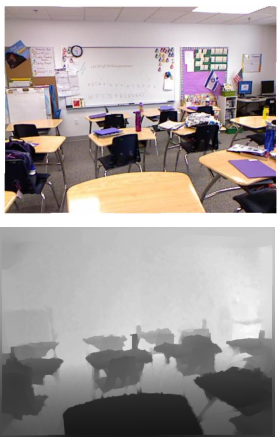
\includegraphics[width=\linewidth]{im2d.png}
\end{block}
\end{column}
\begin{column}{.44\textwidth}
\begin{exampleblock}{Go further}
(2) Build a RGBD CIFAR10 based on indoor depth knowledge\\
\begin{figure}
\includegraphics{../images/207.jpg}
\includegraphics{../train/results/images/207.jpg}
\end{figure}
(3) Compare RGBD and RGB\\
$label=f(RGBD)$
$label=f(RGB)$
\end{exampleblock}
\end{column}
\end{columns}
\end{alertblock}
\end{frame}


\begin{frame}
\frametitle{first part: implement previous work}
\Huge{\centerline{infer depth from RGB image}}
\end{frame}

\begin{frame}
\frametitle{Infer depth from RGB image: Loss defination}
At training time, we combine two objective function\footcite{liu2015deep}
\begin{enumerate}
\item regress to groud truth depth image(Kinect, PrimeSense)
$ \Sigma_{p}(y_p-\hat{y}_p)^2$, p stands for pixel.
\item Similarity between superpixels.
$R_{pq} = \sum_{k=1}^K \beta_k S_{pq}^{(k)}$\\
 $\beta$ is trainable weight. S is similarity function.
\end{enumerate}
\end{frame}


\begin{frame}
\frametitle{Infer depth from RGB image: Architecture}
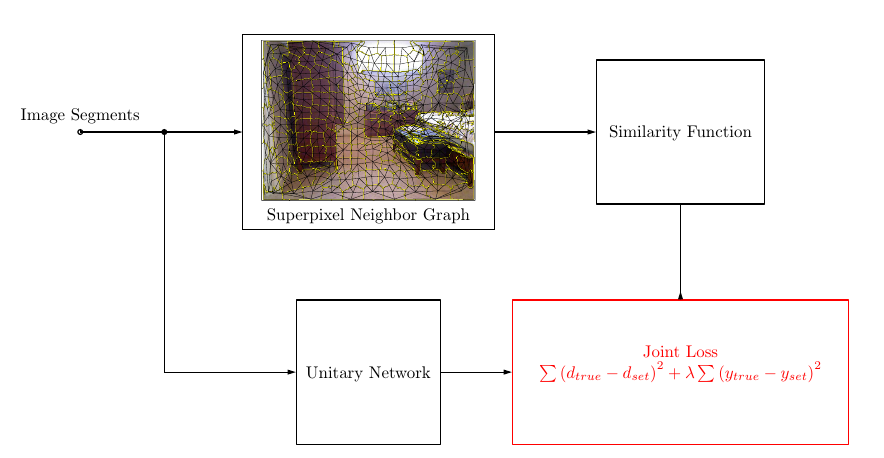
\includegraphics[width=\linewidth]{arch.png}
using traditional CNN.
\end{frame}


\begin{frame}
\frametitle{Infer depth from RGB image: Supervised part}
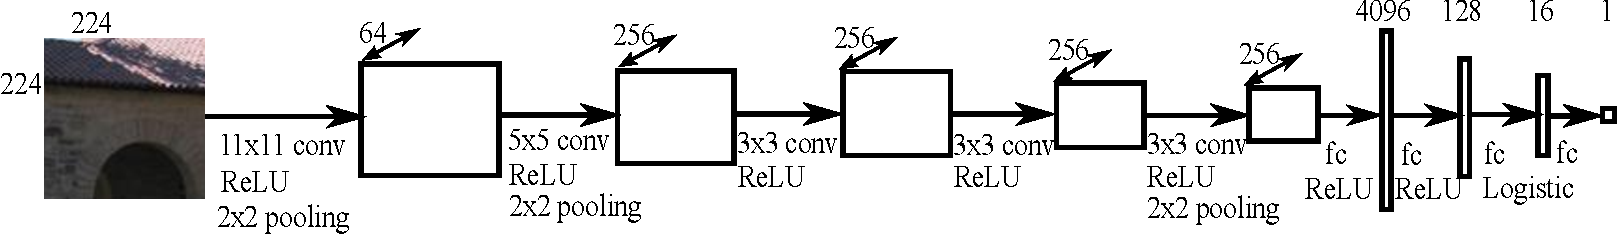
\includegraphics[width=\linewidth]{fig/cnn_unary.pdf}
\end{frame}


\begin{frame}
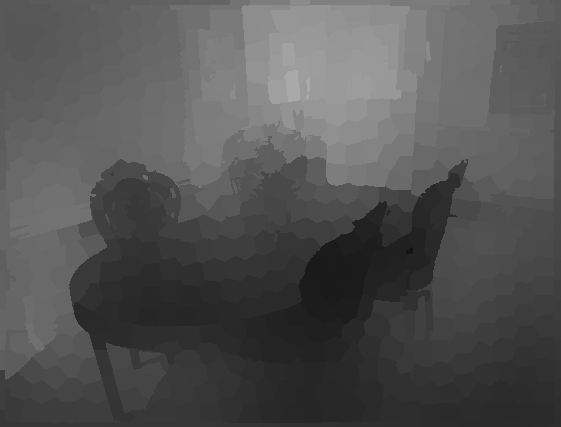
\includegraphics[width=.3\linewidth]{fig/Make3D/image/5.jpg}
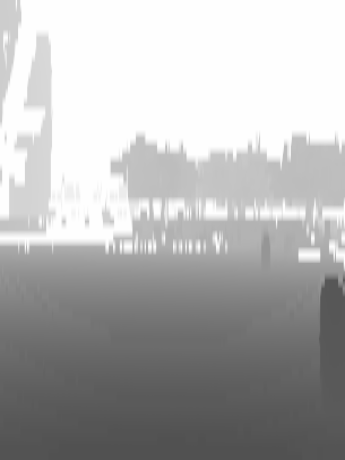
\includegraphics[width=.3\linewidth]{fig/Make3D/gt/5.png}
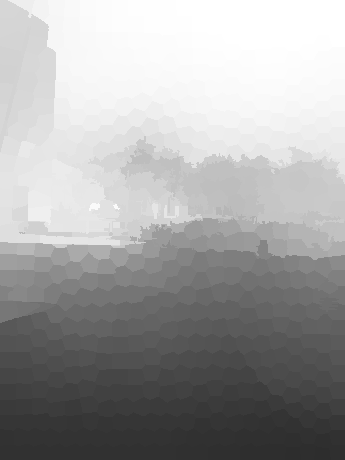
\includegraphics[width=.3\linewidth]{fig/Make3D/ccnf_struct_ft/5.png}\\
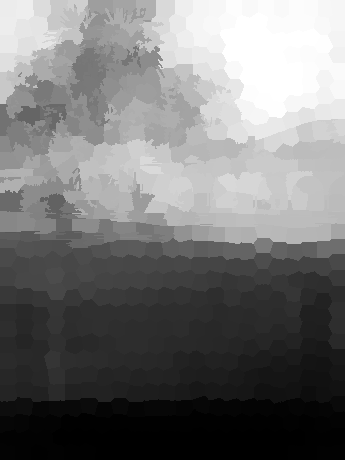
\includegraphics[width=.3\linewidth]{fig/Make3D/image/81.jpg}

\includegraphics[width=.3\linewidth]{fig/Make3D/gt/81.png}
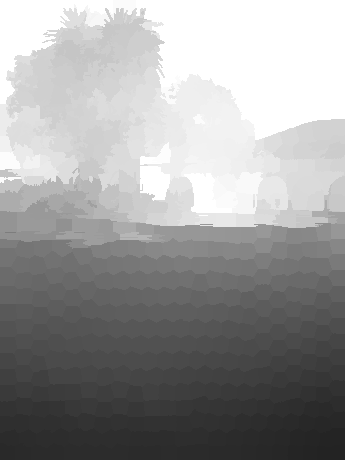
\includegraphics[width=.3\linewidth]{fig/Make3D/ccnf_struct_ft/81.png}\\
\end{frame}


\begin{frame}
\frametitle{Compare performance with original paper}
\begin{table} [t] \center
\resizebox{\linewidth}{!} {
\begin{tabular}{ | l |  c  c  c | c  c  c |}
\hline 
\multirow{3}{*}{{{Method}}} &\multicolumn{3}{c|}{Error} &\multicolumn{3}{c|}{Accuracy} \\
&\multicolumn{3}{c|}{(lower is better)} &\multicolumn{3}{c|}{(higher is better)} \\
\cline{2-7}
&rel &log10 &rms &$\delta < 1.25$ &$\delta < 1.25^2$ &$\delta < 1.25^3$  \\
\hline
%
%
Our implementation &\textbf{0.252}	 &0.103	  &0.860  	&0.544   	&\textbf{0.861}	&0.943  \\
Original paper    &0.230	 &\textbf{0.095} 	 &\textbf{0.824}  &\textbf{0.614} 	 &0.883	 &\textbf{0.971} \\
\hline
\end{tabular}
}
\end{table}
(\textbf{Bold} is better.)
\end{frame}


\begin{frame}
\frametitle{second part: go further}
\Huge{\centerline{Classification on RGBD images}}
\end{frame}


\begin{frame}
\frametitle{build RGBD CIFAR dataset}
\begin{columns}
\begin{column}{.3\textwidth}
\includegraphics{../images/207.jpg}\\
\includegraphics[scale=3]{../images/207.jpg}\\
$400x400x3$
\end{column}

\begin{column}{.2\textwidth}
Through our trained depth estimation model
\end{column}
\begin{column}{.4\textwidth}
\includegraphics[scale=3]{../train/results/images/207.jpg}\\
$400x400x1$\\
\includegraphics{../train/results/images/207.jpg}
\includegraphics{../images/207.jpg}\\
$32x32x4$
\end{column}
\end{columns}
\end{frame}




\begin{frame}
\includegraphics{../images/14945.jpg}
\includegraphics{../train/results/images/14945.jpg}
\includegraphics{../images/115.jpg}
\includegraphics{../train/results/images/115.jpg}
\includegraphics{../images/207.jpg}
\includegraphics{../train/results/images/207.jpg}
\includegraphics{../images/104.jpg}
\includegraphics{../train/results/images/104.jpg}
\includegraphics{../images/29.jpg}
\includegraphics{../train/results/images/29.jpg}\\
\includegraphics{../images/41.jpg}
\includegraphics{../train/results/images/41.jpg}
\includegraphics{../images/108.jpg}
\includegraphics{../train/results/images/108.jpg}
\includegraphics{../images/119.jpg}
\includegraphics{../train/results/images/119.jpg}
\includegraphics{../images/122.jpg}
\includegraphics{../train/results/images/122.jpg}
\includegraphics{../images/123.jpg}
\includegraphics{../train/results/images/123.jpg}\\
\includegraphics{../images/129.jpg}
\includegraphics{../train/results/images/129.jpg}
\includegraphics{../images/131.jpg}
\includegraphics{../train/results/images/131.jpg}
\includegraphics{../images/140.jpg}
\includegraphics{../train/results/images/140.jpg}
\includegraphics{../images/160.jpg}
\includegraphics{../train/results/images/160.jpg}
\includegraphics{../images/182.jpg}
\includegraphics{../train/results/images/182.jpg}\\
\includegraphics{../images/194.jpg}
\includegraphics{../train/results/images/194.jpg}
\includegraphics{../images/213.jpg}
\includegraphics{../train/results/images/213.jpg}
\includegraphics{../images/220.jpg}
\includegraphics{../train/results/images/220.jpg}
\includegraphics{../images/221.jpg}
\includegraphics{../train/results/images/221.jpg}
\includegraphics{../images/240.jpg}
\includegraphics{../train/results/images/240.jpg}\\
\includegraphics{../images/246.jpg}
\includegraphics{../train/results/images/246.jpg}
\includegraphics{../images/264.jpg}
\includegraphics{../train/results/images/264.jpg}
\includegraphics{../images/273.jpg}
\includegraphics{../train/results/images/273.jpg}
\includegraphics{../images/278.jpg}
\includegraphics{../train/results/images/278.jpg}
\includegraphics{../images/284.jpg}
\includegraphics{../train/results/images/284.jpg}\\
\includegraphics{../images/293.jpg}
\includegraphics{../train/results/images/293.jpg}
\includegraphics{../images/295.jpg}
\includegraphics{../train/results/images/295.jpg}
\includegraphics{../images/315.jpg}
\includegraphics{../train/results/images/315.jpg}
\includegraphics{../images/310.jpg}
\includegraphics{../train/results/images/310.jpg}
\includegraphics{../images/341.jpg}
\includegraphics{../train/results/images/341.jpg}\\
\includegraphics{../images/340.jpg}
\includegraphics{../train/results/images/340.jpg}
\includegraphics{../images/371.jpg}
\includegraphics{../train/results/images/371.jpg}
\includegraphics{../images/370.jpg}
\includegraphics{../train/results/images/370.jpg}
\includegraphics{../images/397.jpg}
\includegraphics{../train/results/images/397.jpg}
\includegraphics{../images/414.jpg}
\includegraphics{../train/results/images/414.jpg}\\
\includegraphics{../images/29787.jpg}
\includegraphics{../train/results/images/29787.jpg}
\includegraphics{../images/34731.jpg}
\includegraphics{../train/results/images/34731.jpg}
\includegraphics{../images/34732.jpg}
\includegraphics{../train/results/images/34732.jpg}
\includegraphics{../images/39678.jpg}
\includegraphics{../train/results/images/39678.jpg}
\includegraphics{../images/39679.jpg}
\includegraphics{../train/results/images/39679.jpg}
\end{frame}


\begin{frame}
\frametitle{architecture}
\begin{columns}
\begin{column}{.01\textwidth}
\includegraphics{../images/207.jpg}\\
\includegraphics{../train/results/images/207.jpg}\\
$32x32x4$
\end{column}
\begin{column}{.4\textwidth}
\includegraphics[width=\linewidth]{mp1.png}
\end{column}
\begin{column}{.2\textwidth}
\includegraphics[width=\linewidth]{label.png}
\end{column}
\end{columns}
\end{frame}




\begin{frame}
\frametitle{R vs G vs B vs D: training time}
\includegraphics[width=\linewidth]{train.eps}
\end{frame}


\begin{frame}
\frametitle{R vs G vs B vs D: testing time}
\includegraphics[width=\linewidth]{test.eps}
\end{frame}


\begin{frame}
\frametitle{RGBD vs RGB: training time}
\includegraphics[width=\linewidth]{together_train.eps}
\end{frame}


\begin{frame}
\frametitle{RGBD vs RGB: tges time}
\includegraphics[width=\linewidth]{together_test.eps}
\end{frame}


\begin{frame}
\Huge{\centerline{questions?\footnote{code, references, report, slides can be access here:
\href{https://github.com/yihui-he/Depth-estimation-with-neural-network}{https://github.com/yihui-he/Depth-estimation-with-neural-network}}}}

\end{frame}
%----------------------------------------------------------------------------------------

\end{document}